%====================================================================%
%                  MORIOND.TEX                                       %
%====================================================================%

\documentclass{moriond}

% for BibTeX - sorted numerical labels by order of
% first citation.

% A useful Journal macro
\def\Journal#1#2#3#4{{#1} {\bf #2}, #3 (#4)}

% Some useful journal names
\def\NCA{\em Nuovo Cimento}
\def\NIM{\em Nucl. Instrum. Methods}
\def\NIMA{{\em Nucl. Instrum. Methods} A}
\def\NPB{{\em Nucl. Phys.} B}
\def\PLB{{\em Phys. Lett.}  B}
\def\PRL{\em Phys. Rev. Lett.}
\def\PRD{{\em Phys. Rev.} D}
\def\ZPC{{\em Z. Phys.} C}
\def\apj{{\em Astrophys. J.}}
\def\apjs{{\em Astrophys. J. Suppl.}}
\def\aap{{\em Astron. Astrophys.}}

% Some other macros used in the sample text
\def\st{\scriptstyle}
\def\sst{\scriptscriptstyle}
\def\mco{\multicolumn}
\def\epp{\epsilon^{\prime}}
\def\vep{\varepsilon}
\def\ra{\rightarrow}
\def\ppg{\pi^+\pi^-\gamma}
\def\vp{{\bf p}}
\def\ko{K^0}
\def\kb{\bar{K^0}}
\def\al{\alpha}
\def\ab{\bar{\alpha}}
\def\be{\begin{equation}}
\def\ee{\end{equation}}
\def\bea{\begin{eqnarray}}
\def\eea{\end{eqnarray}}
\def\CPbar{\hbox{{\rm CP}\hskip-1.80em{/}}}
%temp replacement due to no font

\newcommand{\aism}[1]{\textcolor{red}{{AISM:} #1}}
\def\Commander{\texttt{Commander} }
\def\commanderone{\texttt{Commander1} }
\def\commandertwo{\texttt{Commander2} }
\def\commanderthree{\texttt{Commander3} }
\def\commanderfour{\texttt{Commander4} }
\def\WMAP{\textit{WMAP}}
\def\Planck{\textit{Planck}}


%%%%%%%%%%%%%%%%%%%%%%%%%%%%%%%%%%%%%%%%%%%%%%%%%%
%                                                %
%    BEGINNING OF TEXT                           %
%                                                %
%%%%%%%%%%%%%%%%%%%%%%%%%%%%%%%%%%%%%%%%%%%%%%%%%%

%\newcommand{\Photo}{\includegraphics[height=35mm]{mypicture}}
\newcommand{\Photo}{}

\begin{document}
\vspace*{4cm}
\title{Cosmoglobe: Mapping the Universe from the Milky Way to the Big Bang\\\aism{Alternative 1: Cosmoglobe: Past, Present and Future}\\\aism{Alternative 2: Cosmoglobe: A Brief History}}


\author{ A.I. Silva Martins, Cosmoglobe Collaboration\\\aism{they specifically said to not list the whole collaboration, but here it probably makes sense to list some other people, maybe the first authors of the overview papers, including obvisouly Ingunn since this was her ERC and HK since Commander was his idea}}

\address{Institute of Theoretical Astrophysics, University of Oslo, Sem Sælands vei 13,\\
0371 Oslo, Norway}

\maketitle\abstracts{
This is where the abstract should be placed. It should consist of one paragraph
and give a concise summary of the material in the article below.
Replace the title, authors, and addresses within the curly brackets
with your own title, authors, and addresses; please use
capital letters for the title and the authors. You may have as many authors and
addresses as you wish. It's preferable not to use footnotes in the abstract
or the title; the
acknowledgments for funding bodies etc.are placed in a separate section at
the end of the text.}

\section{Introduction}

The idea behind the Cosmoglobe project is very simple: if all of the instruments we have built so far and are in the process of building are looking at the same sky, then, when analysed together, these should have an underlying signal in common. By jointly analysing these datasets, we can better constrain both this underlying signal, as well as any instrumental or otherwise systematic effects, that could otherwise be mistaken for cosmological signal. This allows us to take advantage of the complementarity of the different datasets.

In order to do this, we use a Bayesian end-to-end analysis framework, called \Commander\footnote{Originally named this way as it was meant to be used in combination with the Master algorithm~\cite{hivon:2002}, and after the at the time famous film: Master and Commander. Also meant to be an acronym for ``Commander is an Optimal Monte-carlo Markov chAiN Driven EstimatoR''.}~\cite{eriksen:2004,seljebotn:2019,bp03}. \Commander\ is a Gibbs sampling code, which allows us to sample from the full joint posterior distribution of all the parameters in our model, including both the cosmological signal and the instrumental parameters, as shown in Figure~\ref{fig:cosmoglobe}. This allows us to propagate uncertainties in a consistent way, and to marginalize over any nuisance parameters.

\begin{figure}[htb]
\centerline{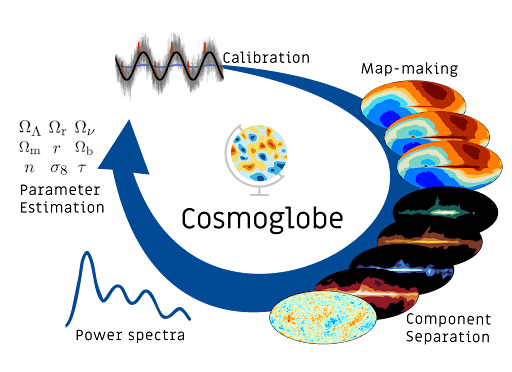
\includegraphics[width=0.7\linewidth]{figures/cosmoglobe.png}}
\caption[]{The Cosmoglobe loop. We start with calibrating each of the different datasets; then, making maps of the sky at each frequency that each experiment is observing; then, separating the sky into its different components, e.g. CMB, dust, free-free, AME, synchrotron, etc; then, we produce power spectra; and we are able to estimate the values of cosmological parameters from these. Finally, we do it all over again, using what we have learned in the previous iteration to better calibrate the data, and so on, until we have converged to a stable solution.}
\label{fig:cosmoglobe}
\end{figure}

\aism{add bayes etc equations?}

\subsection{\commanderone}

\commanderone, or, at the time, simply \Commander, was first developed as a means for power spectrum estimation for the high resolution maps produced by the \WMAP\ mission~\cite{bennett:2013}. It was later used as one of the main component separation frameworks for the analysis of the \Planck\ data~\cite{planck2014-a12}. A particularly useful feature of \commanderone\ is the ability to sample spatially variable spectral indices~\cite{fuskeland2014}. The \commanderone\ code was developed in Fortran and is not publicaly available. \aism{should we use this as an opportunity to add commander 1 and 2 to the github?}

\subsection{\commandertwo}

\commandertwo\ is the second generation of the \Commander\ framework, designed to be able to do everything \commanderone\ could do, including now also support for multi-resolution datasets. The code \commandertwo\ code was also developed in Fortran and is also not publicaly available.

\subsection{\commanderthree}

\Commander\ suffered a major rewrite in between its second and third generations, with \commanderthree\ now being able to perform end-to-end analysis, starting from the raw data, all the way to parameter estimation. The \commanderthree\ code is written in Fortran and is publicaly available on GitHub\footnote{\url{https://github.com/Cosmoglobe/Commander}}. It is also still maintained and developed at the time of writting.

\subsection{\commanderfour}
\commanderfour\ is the latest generation of the \Commander\ framework, which, once again, meant a major rewrite of the \Commander\ code, in order to be able to efficiently paralelize the code and to be able to run on modern high performance computing architectures, so that we can handle larger, new generation datasets. The differences between the architectures of \commanderthree\ and \commanderfour\ are outlined in Figure~\ref{fig:commander4}. \commanderfour\ is also designed to be more modular and flexible than its predecessors, specifically to allow new contributors to easily analyse their own datasets using it or even add new features. \commanderfour\ is currently being developed in Python and is publicaly available on GitHub\footnote{\url{https://github.com/Cosmoglobe/Commander4}}.

\begin{figure}[htb]
\centerline{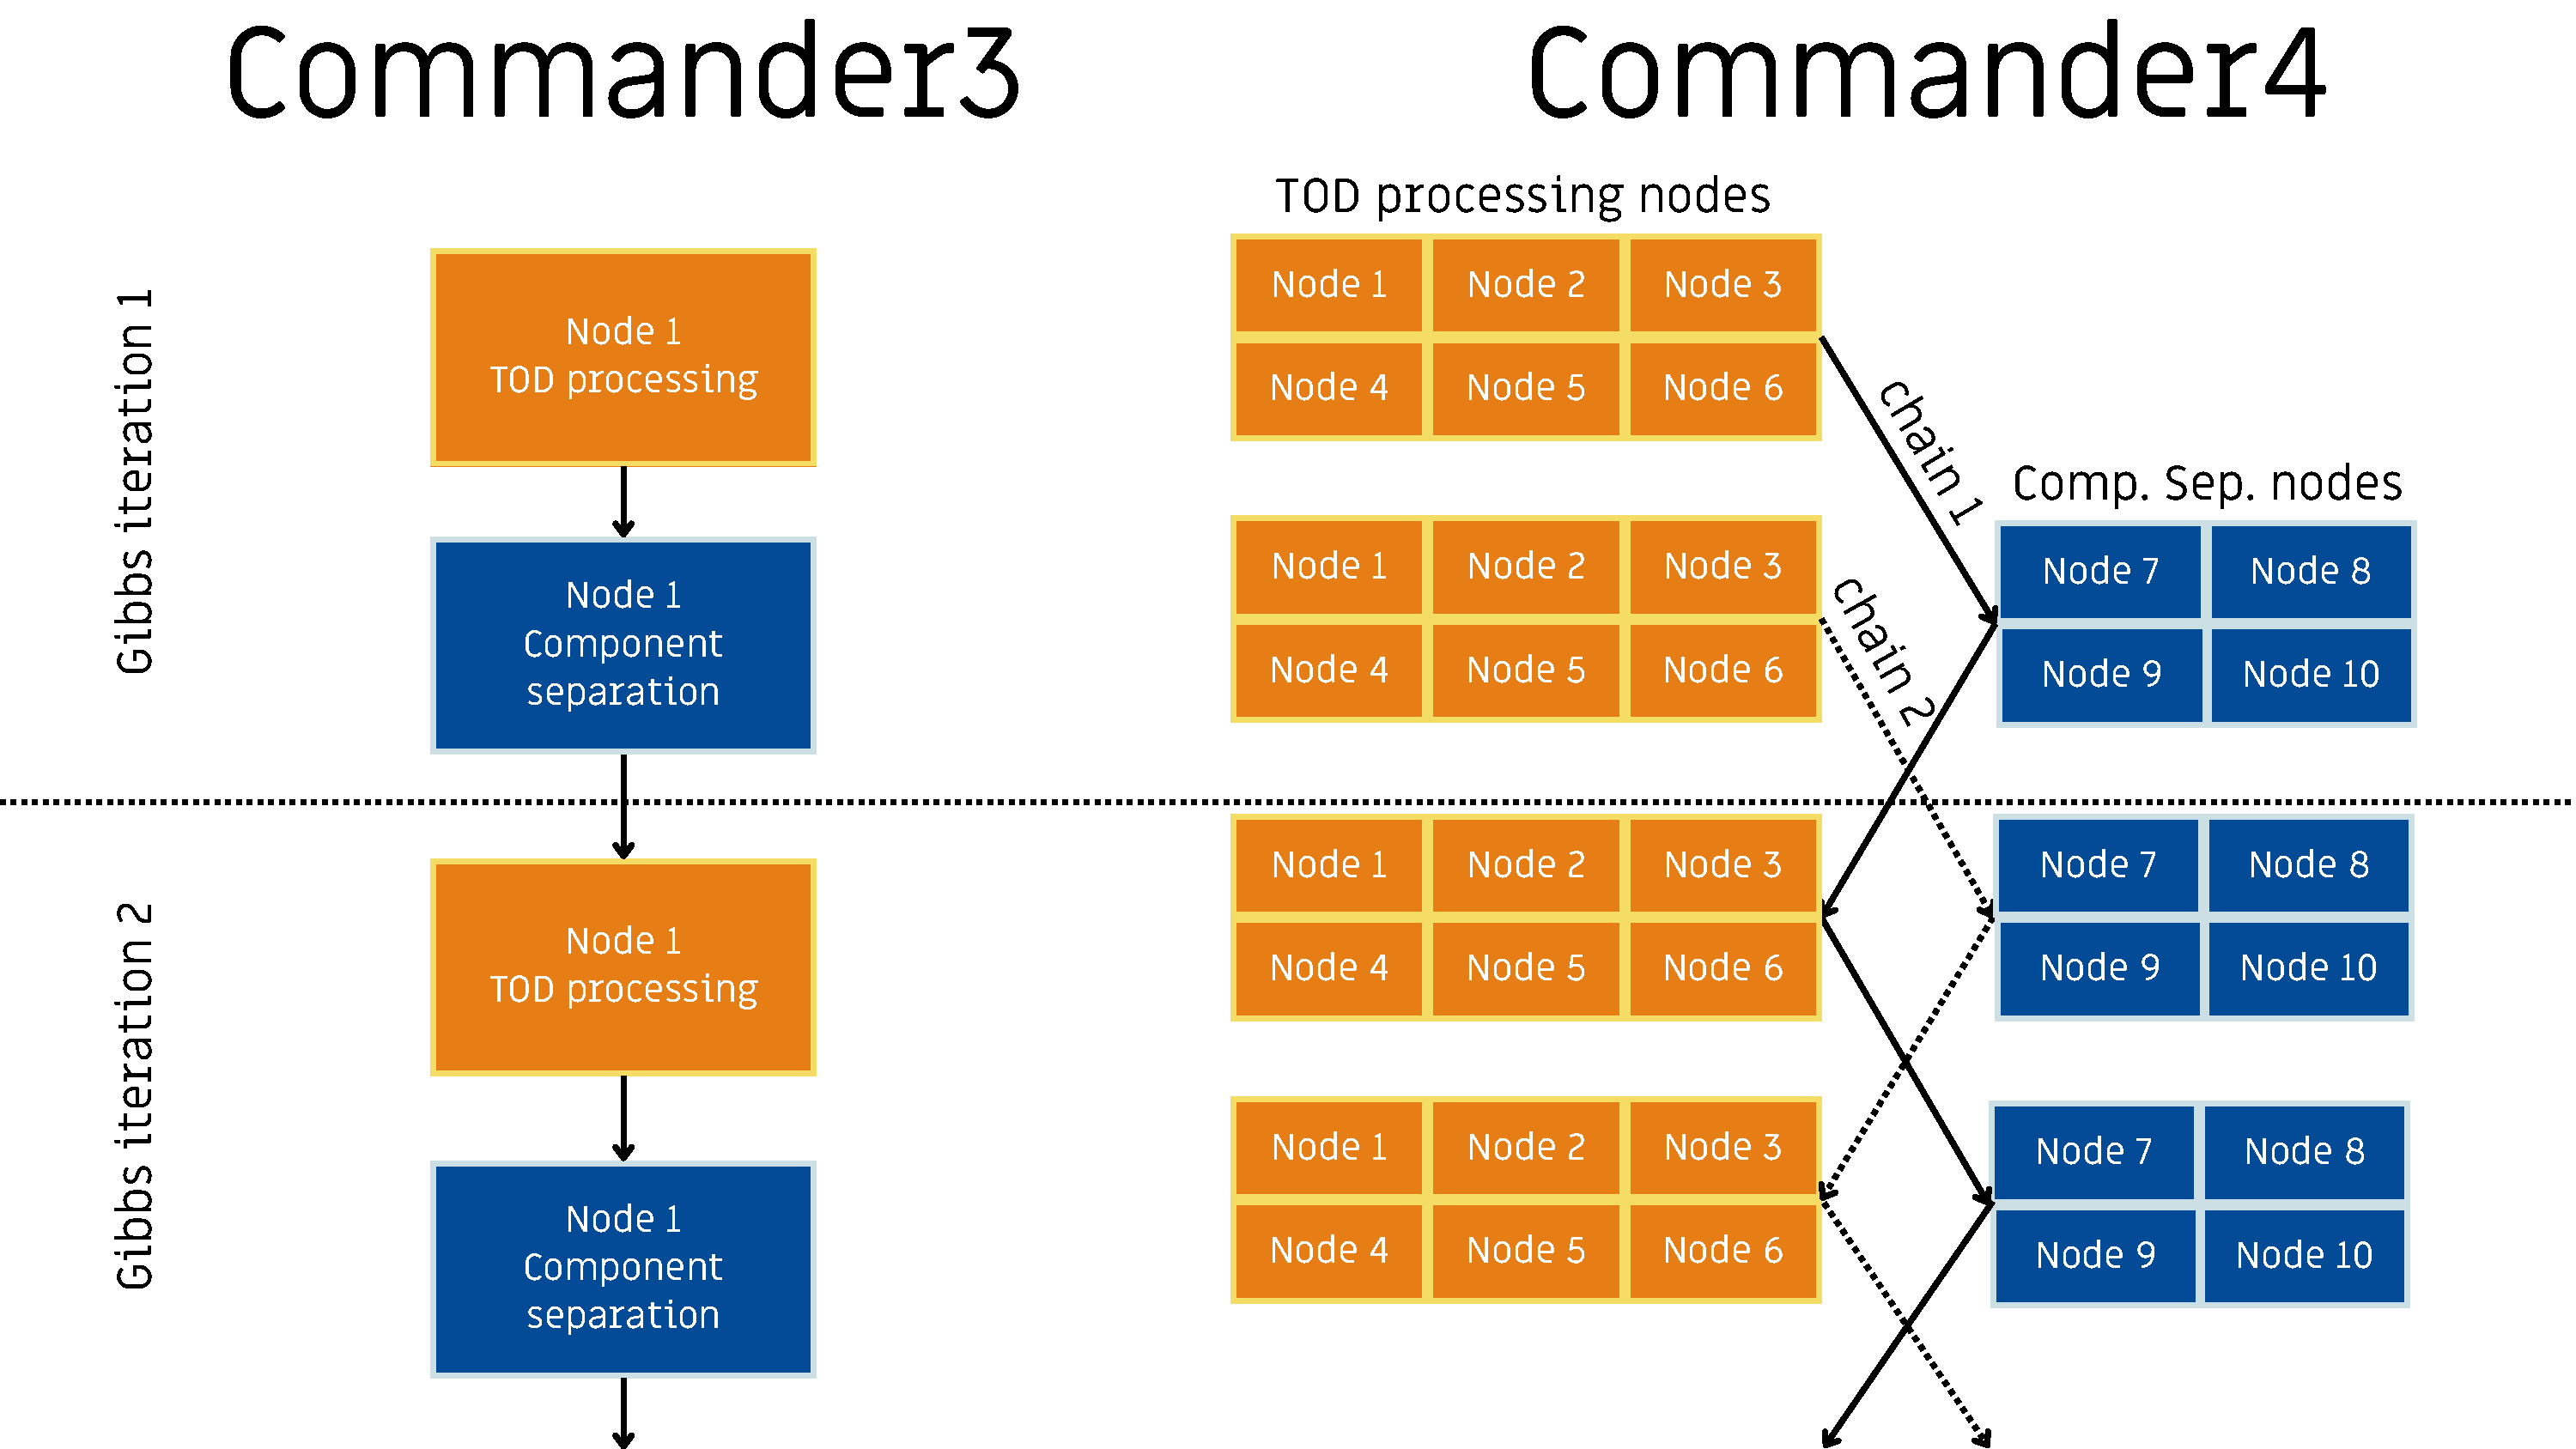
\includegraphics[width=\linewidth]{figures/commander4.pdf}}
\caption[]{While \commanderthree\ has a linear architecture, only being able to parallelize tasks within one node, \commanderfour\ is able to paralelize tasks across multiple nodes. In this scheme, we show dedicated nodes for each step in the analysis, which also allows us to run a second Markov chain at the same time, taking advantage of all of the nodes at all times, and being left with more Gibbs iterations to infer our parameters and their uncertainties from.}
\label{fig:commander4}
\end{figure}

\begin{table}[t]
\caption[]{Experimental Data bearing on $\Gamma(K \ra \pi \pi \gamma)$
for the $\ko_S, \ko_L$ and $K^-$ mesons.}
\label{tab:exp}
\vspace{0.4cm}
\begin{center}
\begin{tabular}{|c|c|c|l|}
\hline
& & & \\
&
$\Gamma(\pi^- \pi^0)\; s^{-1}$ &
$\Gamma(\pi^- \pi^0 \gamma)\; s^{-1}$ &
\\ \hline
\mco{2}{|c|}{Process for Decay} & & \\
\cline{1-2}
$K^-$ &
$1.711 \times 10^7$ &
\begin{minipage}{1in}
$2.22 \times 10^4$ \\ (DE $ 1.46 \times 10^3)$
\end{minipage} &
\begin{minipage}{1.5in}
No (IB)-E1 interference seen but data shows excess events relative to IB over
$E^{\ast}_{\gamma} = 80$ to $100MeV$
\end{minipage} \\
& & &  \\ \hline
\end{tabular}
\end{center}
\end{table}

\section{BeyondPlanck}

\begin{equation}
\renewcommand{\arraystretch}{1.2}
\begin{array}{rc@{\,}c@{\,}l}
%\begin{array}{>{\displaystyle}r>{\displaystyle}c>{\displaystyle}c>{\displaystyle}l}

%\begin{eqnarray}
\bf{K} & = &&  Im[V_{j, \alpha} {V_{j,\alpha + 1}}^*
{V_{j + 1,\alpha }}^* V_{j + 1, \alpha + 1} ] \\
%       &   & + & Im[V_{k, \alpha + 2} {V_{k,\alpha + 3}}^*
%{V_{k + 1,\alpha + 2 }}^* V_{k + 1, \alpha + 3} ]  \\
       &   & + & Im[V_{j + 2, \beta} {V_{j + 2,\beta + 1}}^*
{V_{j + 3,\beta }}^* V_{j + 3, \beta + 1} ]  \\
       &   & + & Im[V_{k + 2, \beta + 2} {V_{k + 2,\beta + 3}}^*
{V_{k + 3,\beta + 2 }}^* V_{k + 3, \beta + 3}] \\
& & \\
\bf{M} & = &&  Im[{V_{j, \alpha}}^* V_{j,\alpha + 1}
V_{j + 1,\alpha } {V_{j + 1, \alpha + 1}}^* ]  \\
%       &   & + & Im[V_{k, \alpha + 2} {V_{k,\alpha + 3}}^*
%{V_{k + 1,\alpha + 2 }}^* V_{k + 1, \alpha + 3} ]  \\
       &   & + & Im[{V_{j + 2, \beta}}^* V_{j + 2,\beta + 1}
V_{j + 3,\beta } {V_{j + 3, \beta + 1}}^* ]  \\
       &   & + & Im[V_{k + 2, \beta + 2} {V_{k + 2,\beta + 3}}^*
{V_{k + 3,\beta + 2 }}^* V_{k + 3, \beta + 3}],
\\ & &
\end{array}
%\end{eqnarray}
\label{eq:spa}
\end{equation}

\begin{figure}
\begin{minipage}{0.20\linewidth}
%\centerline{\includegraphics[width=0.7\linewidth,draft=true]{figexamp}}
\end{minipage}
\hfill
\begin{minipage}{0.20\linewidth}
%\centerline{\includegraphics[width=0.7\linewidth]{figexamp}}
\end{minipage}
\hfill
\begin{minipage}{0.20\linewidth}
%\centerline{\includegraphics[angle=-45,width=0.7\linewidth]{figexamp}}
\end{minipage}
\caption[]{same figure with draft option (left), normal (center) and rotated (right)}
\label{fig:radish}
\end{figure}

\section{Data Release 1}

\section{Data Release 2}

\section{Current Status and Future Prospects}

\section*{Acknowledgments}


\section*{Appendix}


\section*{References}
\bibliography{moriond}

%%% manually generated bibliography
%\begin{thebibliography}{99}
%\bibitem{ja}C Jarlskog in {\em CP Violation}, ed. C Jarlskog
%(World Scientific, Singapore, 1988).
%\bibitem{ma}L. Maiani, \Journal{\PLB}{62}{183}{1976}.
%\bibitem{bu}J.D. Bjorken and I. Dunietz, \Journal{\PRD}{36}{2109}{1987}.
%\bibitem{bd}C.D. Buchanan {\it et al}, \Journal{\PRD}{45}{4088}{1992}.
%\end{thebibliography}

\end{document}

%%%%%%%%%%%%%%%%%%%%%%
% End of moriond.tex  %
%%%%%%%%%%%%%%%%%%%%%%


%%% Local Variables: 
%%% mode: latex
%%% TeX-master: t
%%% End: 
